\documentclass[crop,tikz]{standalone}
\usetikzlibrary{positioning,arrows,fit,calc}
\pgfdeclarelayer{bg}
\pgfsetlayers{bg,main}
\tikzset{
	>=stealth'
}
\begin{document}
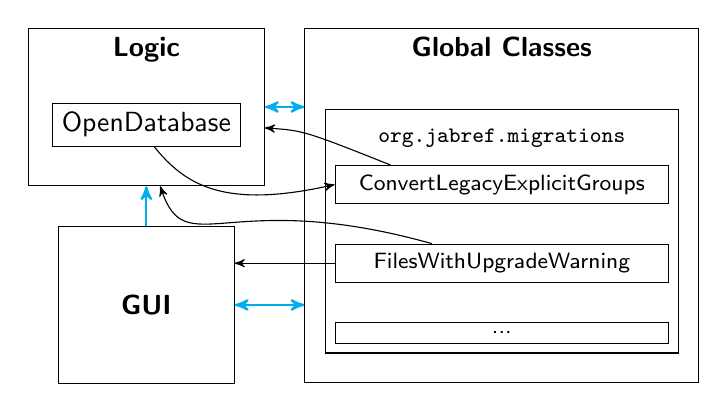
\begin{tikzpicture}[
node distance = 5mm,
every node/.style = {
	font = \sffamily
}, 
component title/.style = {
	font = \bfseries\sffamily
},
component/.style = {
	component title,
	draw, 
	minimum height = 2cm,
	text width = 2cm,
	align = center
},
cmpdep/.style = {
	->,
	thick,
	cyan
},
pkg/.style = {
	font = \footnotesize\ttfamily
},
small class/.style = {
	font = \footnotesize\sffamily,
	draw,
	text width = 4cm,
	align = center
}
]

\node [component, minimum width=3cm] (logic) {};
\node [component title, below = 0mm of logic.north] {Logic};

\node [draw, above = of logic.south] (od) {OpenDatabase};

\node [component, below = of logic] (gui) {GUI};

\node [component, right = of logic.north east, anchor = north west, minimum height = 4.5cm, minimum width = 5cm] (global) {};
\node [component title, below = 0mm of global.north] {Global Classes};

\node [small class, above = of global.south] (other) {...};
\node [small class, above =  of other] (fwuw) {FilesWithUpgradeWarning};
\node [small class, above =  of fwuw] (cleg) {ConvertLegacyExplicitGroups};

\node [pkg, above = 1mm of cleg] (pkg) {org.jabref.migrations};
\node [draw, fit = {
	(fwuw)
	(cleg)
	(other)
	(pkg)
}] {};

\draw[->] (od.290) .. controls (0.5,-1) and (1,-1.3) .. (cleg.180);
\draw[->] (cleg.170) .. controls (2, -0.3)  .. (logic.350);

\draw[->] (fwuw) -- (fwuw -| gui.east);
\draw[->] (fwuw) .. controls (1, -1) and (0.5, -2) .. (logic.280);

\draw[cmpdep] (gui) -- (logic);
\draw[cmpdep, <->] (gui) -- (gui -| global.west);
\draw[cmpdep, <->] (logic) -- (logic -| global.west);

\end{tikzpicture}

\end{document}